\section{Apache S4}


Nach der Vorstellung von Apache Storm, Kafka und Flume wird in diesem Kapitel Apache S4 vorgestellt. Apache S4 ist eine Abkürzung und steht für Simple Scalable Streaming System und wird von Flavio Junqueira als allgemeine, verteilte, skalierbare, teilweise fehlertolerante und steckbare Plattform bezeichnet \citeint{s4:Proposal}. Zunächst soll eine Kurzübersicht einen ersten Einblick in Apache S4 geben. Anschließend werden die Bewertungskriterien erläutert und vorgestellt.

\begin{table}[tbp]
	\centering
		\begin{tabular}{@{}ll@{}} \toprule
			\textbf{Faktum} & \textbf{Beschreibung} \\ \midrule
			Hauptentwickler & Matthieu Morel, Kishore Gopalakrishna, Flavio Junqueira \\
			& Leo Neumeyer, Bruce Robbins, Daniel Gomez Ferro \\
			Stabile Version & 0.6.0 vom 03.06.2013 \\ 
			Entwicklungsstatus &  Moderat \\
			Entwicklungsversion & 0.7.0 \\
			Sprache & Java \\
			Betriebssystem & plattformunabhängig, benötigt die Java Virtual Machine \\
			& und Apache Zookeeper \\
			Lizenz & Apache License version 2.0 \\
			Webseite & \citeint{s4:home} \\
			Quelltext & \citeint{s4:GitHubApacheMirror} \\			
			\bottomrule			
		\end{tabular}
	\caption{Kurzübersicht Apache S4}
	\label{tab:vors4}
\end{table}


Die Architektur von Apache S4 baut auf einem Apache Zookeeper Cluster auf und besteht aus mehreren Apache S4 \textit{Cluster}, \textit{Processing Nodes}, \textit{Apps}, \textit{Processing Elements} und dem \textit{Communication Layer}. \textit{Apps} sind Java Archive die in einem Apache S4 \textit{Cluster} bereitgestellt werden. Die Größe eines \textit{Clusters} entspricht der Anzahl der \textit{Tasks}. Pro \textit{Task} muss jeweils eine \textit{Processing Node} als selbständiger Prozess gestartet werden. Eine \textit{Procssing Node} dient als Container für mehrere \textit{Processing Elements}. \textit{Apps} bestehen aus einem Graphen von \textit{Processing Elements} und \textit{Streams}. Ein \textit{Processing Element} kommuniziert asynchron über unterschiedliche \textit{Cluster} per \textit{Streams}. Der Nachrichtenaustausch erfolgt über den \textit{Communication Layer}. Abbildung \ref{fig:s4ProcessingNode} zeigt Zwei Processing Nodes mit mehreren Processing Elements. Ein Raw Event wird von der äußeren Umgebung an die erste Processing Node in den Event Listener übergeben. Der Dispatcher erhält die verarbeitete Nachricht von einem Processing Element und leitet diese an den Emitter weiter. Der Emitter setzt die Nachricht in einen Stream. Der Stream wird vom Communication Layer an die zweite Processing Node vermittelt. Die Verarbeitung wird von der zweiten Processing Node durchgeführt. Das User Interface Model holt sich die Nachrichten vom neuen Stream ab und stellt die Information in der Benutzerschnittstelle dar.

Eine spezielle Implementierung einer Nachricht muss von der Klasse \textit{Event} erben, aus einem Schlüssel/Wert-Tupel bestehen und an einen \textit{Stream} weitergegeben werden können. Mit der Erweiterung der Basisklasse \textit{AdapterApp} kann ein \textit{Stream} erzeugt werden. Ein Beispiel wird im Anhang \ref{lst:s4HelloInputAdapter} gezeigt. Dabei wird auf eine Netzwerkverbindung mit dem Anschluss 15000 gehört. Bei erfolgreicher Verbindung wird der Inhalt gelesen und in einen \textit{Stream} gesetzt. 

\begin{figure}[htb!]
\centering
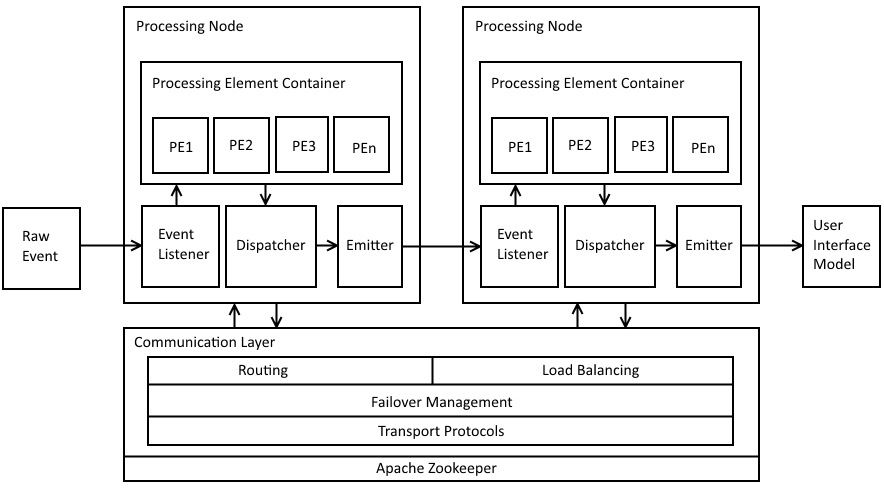
\includegraphics[width=1.0\textwidth]{bilder/s4ProcessingNodes.png}
\caption{Apache S4 Processing Nodes
\label{fig:s4ProcessingNode}}
\end{figure}

In einem \textit{Processing Element} wird die Datenverarbeitung durchgeführt. In Apache S4 gibt es nur zwei Typen von \textit{Processing Elements}, ein Schlüssel-loses und ein Schlüssel-behaftetes \textit{Processing Element}. Der Schlüssel-lose Typ kann unterschiedliche Apache S4 Nachrichten empfangen. Der Schlüssel-behaftete Typ kann nur Apache S4 Nachrichten mit einem definierten Schlüssel in der Nachricht empfangen. Spezielle Aggregate und Operatoren von Nachrichten müssen in \textit{Processing Elements}-Klassen explizit implementiert werden. Ein \textit{Processing Element} besteht aus Zwei Teilen, dem \textit{Prototype} und der \textit{Instance}. Der \textit{Prototype} erbt von der Basisklasse \textit{ProcessingElement} und behandelt eingehende Nachrichten. Die \textit{Instance} erbt von der Basisklasse \textit{App} und behandelt den Anwendungsstart und Anwendungsstop. Im Anhang \ref{lst:s4HelloAppProcessingElementInstance} wird ein Beispiel für das Erzeugen eines \textit{Streams} "`names"' und die Weitergabe der Nachrichten an einen \textit{Stream} gezeigt. \citeint{s4:overview}

In Abbildung \ref{fig:s4HelloApp} wird das Beispiel \ref{s4:beispielHelloApp} aus der Apache S4 Installation im Anhang \ref{sec:s4install} gezeigt. Die Abbildung \ref{fig:s4HelloApp} wurde aus der Dokumentation \citeint{s4:walkthrough} entnommen. Zuerst werden Zwei Cluster \textit{cluster1} und \textit{cluster2} in einem Apache Zookeeper \textit{Cluster} bereitgestellt. Anschließend wird im \textit{Repository} die S4 Anwendung \textit{myApp} hinzugefügt. Die Apache S4 \textit{Nodes} werden über Apache Zookeeper informiert und die Anwendung wird gestartet. Ein neuer \textit{Stream} "`names"' wird erstellt und beide \textit{Nodes} werden als \textit{Consumer} registriert. Anschließend wird im \textit{Cluster} \textit{cluster2} die \textit{HelloInputAdapter}-Anwendung gestartet. Beim Bereitstellen der Anwendung im \textit{Cluster} \textit{cluster2} wird der \textit{Stream} "'names"' als Identität für den Ausgabestrom gesetzt. Die \textit{HelloInputAdapter}-Anwendung ist nach dem Starten aktiv und wartet auf Dateneingang. Abschließend werden eintreffende Daten vom \textit{Cluster} \textit{cluster2} in Apache S4-Nachrichten umgewandelt und zur weiteren Datenbehandlung an die \textit{Consumer} verteilt.

\begin{figure}[htb!]
\centering
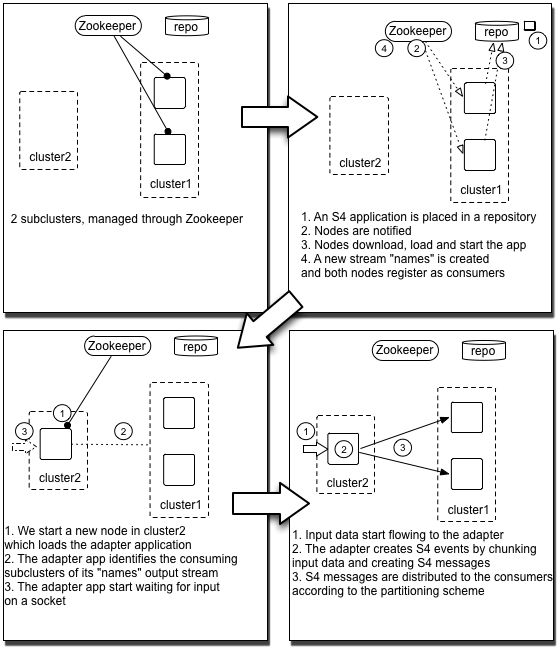
\includegraphics[width=1.0\textwidth]{bilder/s4SampleAppDeployment.png}
\caption{Apache S4 HelloApp Beispiel
\label{fig:s4HelloApp}}
\end{figure}

Nachrichten werden in Apache S4 zwischen den \textit{Nodes} durch den \textit{Communication Layer} übertragen. Der \textit{Communication Layer} nutzt für die Koordination der Nachrichten zwischen den Apache S4 \textit{Nodes} Apache Zookeeper. Um Nachrichten an die \textit{Nodes} im Apache S4 \textit{Cluster} zu senden, können spezielle Bindungen in verschiedenen Programmiersprachen implementiert werden. Durch ein steckbares Design können unterschiedliche Nachrichtenprotokolle wie zum Beispiel Apache Avro oder Apache Thrift eingesetzt werden. Eine Implementierung für das \gls{glo:udp} \citeint{s4:classUdpEmitter} und dem \gls{glo:tcp} \citeint{s4:classTcpEmitter} wird von Apache S4 bereits unterstützt. \citelit[S. 4, Kap. II D]{s4:Neumeyer}

Die Fehlertoleranz in Apache S4 wird durch die \textit{Fail-Fast} Strategie von Apache Zookeeper übernommen. In einem Apache S4 Cluster mit Zwei \textit{Tasks} und Vier gestarteten \textit{Nodes}, sind Zwei \textit{Nodes} Aktiv und Zwei \textit{Nodes} im \textit{Standby}-Betrieb. Wenn Apache Zookeeper einen \textit{Session-Timeout} einer aktiven \textit{Node} feststellt, wird sofort eine \textit{Standby-Node} aktiviert, die anderen \textit{Nodes} werden durch den \textit{Communication Layer} über neue aktive \textit{Node} informiert und neue Nachrichten werden umgeleitet. Apache S4 \textit{Nodes} speichern nutzen für die Datenverarbeitung den lokalen Speicher von Apache Zookeeper. Im Fehlerfall geht der Zwischenspeicher einer Apache Zookeeper \textit{Node} verloren. Damit die Daten nicht verloren gehen, kann mit dem \textit{Checkpointing}-Mechanismus über die Konfiguration eine Datensicherung in einem externen Datenlager erfolgen. Beim Start der neuen \textit{Node} aus dem \textit{Standby}-Betrieb kann die Datensicherung in den lokalen Speicher zurückgeschrieben werden. In \citelit{valles2012analysis} untersucht Vall{\'e}s verschiedene Ansätze von \textit{Checkpointing} und zeigt eine geringe Performanz der Standardimplementierung gegenüber einer Implementierung mit Apache HBase\footnote{Apache HBase ist eine Apache Hadoop Datenbank, ein verteilter, skalierbarer Big Data-Speicher \citeint{hbase:home}.}. \citeint{s4:faultTolerance}

\begin{table}[!ht]
	\centering
		\begin{tabular}{@{}ll@{}} \toprule
			\textbf{Kriterium} & \textbf{Bewertung} \\ \midrule
			Architektur & Strukturierte Peer-to-Peer-Architektur \\
			Prozesse und Threads & Client-Server-Modell \\
			Kommunikation & TCP-basiert und UDP-basiert via Apache Zookeeper \\
			Namenssystem & Hierarchische Benennung \\
			Synchronisierung & Communication Layer \\
			Pipelining und Materialisierung & Chaining von Processing Elements  \\
			Konsistenz und Replikation & Consistent hashing, Checkpointing \\
			Fehlertoleranz & Failover und Checkpointing \\ 
			Sicherheit & Nur eigene Maßnahmen \\
			& Monitoring mit JMX pro Node \\
			Erweiterung & Modulare Eigenentwicklung \\
			Qualität & Nur eigene Entwicklung für \gls{glo:qos}  \\
			\bottomrule			
		\end{tabular}
	\caption{Bewertung Apache S4}
	\label{tab:bews4}
\end{table}

Bei der Sicherheit sind eigene Maßnahmen notwendig. Nachrichten werden im Klartext oder binär übertragen. Die Verbindung zwischen den einzelnen \textit{Processing Nodes} findet unautorisiert statt. Für die Autorisierung und Verschlüsselung ist eine spezielle Implementierung des \textit{Communication Layer} und der einzelnen \textit{Processing Elements} notwendig. Weiterhin ist eine Verschlüsselung des lokalen Speichers von Apache Zookeeper in einem offenen Netz zu empfehlen. Über \gls{glo:jmx} können Metriken eines Apache S4 Clusters abgefragt werden \citeint{s4:metrics}. \gls{glo:qos} wird in \citelit[S. 3, Kap. II B]{s4:Neumeyer} als anwendungsspezifisch eingestuft. In einer spezifischen Anwendung muss daher eine eigene Implementierung für das \gls{glo:qos} in Apache S4, innerhalb von \textit{Processing Elements} erfolgen.


Diese Kapitel stellt das Streaming framework Apache S4 vor. Es wurde auf die Installation von Apache S4 beschrieben und im Anhang \ref{sec:s4install} eine Anleitung abgelegt. Weiterhin wurde die Architektur und der Informationsfluss in einem Apache S4 \textit{Cluster} erläutert. Es wurde die Fehlertoleranz in Zusammenhang von Apache Zookeeper und die Replikation mit \textit{Checkpointing} beschrieben. Zuletzt wurde auf geringe Sicherheit, Monitoring und Qualität hingewiesen. Nach der Vorstellung der Streaming frameworks, werden im folgenden Kapitel die wesentlichen Kernelemente der einzelnen Streaming frameworks zusammengefasst.